% created on 12/05/2020
% @author : ebazan
\chapter{Color image texture analysis based on Gabor features}

In this chapter we present the spectral decomposition of a color image by means of the Gabor filter. We use the theory about Gabor functions developed in Chapter to extract local texture features of a color image. The main strategy consist on from transforming the input image from a three-channel real color space into a two-channel complex color representation. Then, we use a bank of Gabor filters on each channel of the image to extract the texture information generated by the variations of color and illumination in the image.

\section{Introduction}

Gabor filters have long been used for analyzing textures and extracting corresponding image features. Its adaptability and customization depending on the application and the relationship with the human visual system \cite{Daugman:JOSA:1985a}, have made this technique one of the most relevant for the analysis of textures in an image.


The use of Gabor filters for image texture analysis is highly dependent on the final application. Some of the most recognized works in literature date back to the late 90s, where this technique was a hot research topic for image texture analysis. However, regarding the works present in the literature, we can make a clear separation taking into account the nature of the extracted features. The first group uses Gabor filters to extract a global texture descriptor (Gabor signature). Generally this strategy is suitable for applications where the images contain homogeneous textures and it is sought to make the the classification of images or an image retrieval system based on the content, as we can see in Chapter \ref{ch:distance_between_distributions}. The second group is characterized by using Gabor filters to obtain local texture features present in an image. Such a strategy is suitable for image segmentation tasks. In this chapter we address in a detailed and comprehensive way the second case, delving into the spectral decomposition of color images to obtain texture features generated by the changes in illumination and/or color.

In both aforementioned cases of use, we take advantage of the Gabor function's dual-domain (spatial and frequency) representation capability to create a bank of filters $\mathcal{G}=\{g_{f, \theta}(x, y) \}$ that works at different central frequencies $f$ (scales) and orientations $\theta$ to obtain the spectral decomposition of an input image $I(x, y)$ through the convolution operation of each of the filters. 

\begin{equation}\label{eq:gabor_responses}
    r_{f, \theta}(x,y) = I(x, y) \ast g_{f, \theta}(x,y)
\end{equation}

As we know, due to the complex form of Gabor's filters \ref{eq:gabor_function_2d_spacefreq_bank} defined in the chapter \ref{ch:gabor_filter_description}, the response of the filter $r_{f,\theta} (x, y)$ will have, in the same way as the filter, a real part and an imaginary part, here denoted as $\Re{(\cdot)}$ and $\Im{(\cdot)}$, respectively.

The linear transformation of an image using Eq. \eqref{eq:gabor_responses}, produces considerable information about the textures present in the image. The efficient manipulation of this information is the basis for the extraction of appropriate (local or global) texture features. Although this manipulation is a common denominator in techniques based on signal processing, in the literature we can find various schemes to create more separable texture features (see Figure \ref{fig:general_pipeline_gabor_feature_extraction}). In general, these methods vary in the type of output they use to measure the textural information of the image and the post-processing performed

The possible filter responses to measure the texture information are: 

\begin{enumerate}
    \item Amplitude of the response (magnitude or Gabor energy) \cite{Bovik.Clark.ea:TPAMI:1990}
        \begin{equation}\label{eq:gabor_magnitude}
            |r_{f, \theta}(x,y)| = \sqrt{\Re{(r_{f, \theta}(x, y))}^2 + \Im{(r_{f, \theta}(x, y))}^2}
        \end{equation}
    \item Phase of the response \cite{Palm.Lehmann:MGV:2002}
    \begin{equation}\label{eq:gabor_phase}
            \arg(r_{f, \theta}(x,y)) = \arctan2{\left(\frac{\Im{(r_{f, \theta}(x, y))}}{\Re{(r_{f, \theta}(x, y))}}\right)}
        \end{equation}
    \item Real component of the response \cite{Jain.Farrokhnia:IJPR:1991}
    \begin{equation}\label{eq:gabor_real_part}
            \Re{(r_{f, \theta}(x, y))}
        \end{equation}
    \item Square amplitude of the response (Gabor local power spectrum) \cite{Grigorescu.Petkov.ea:TIP:2002}
    \begin{equation}\label{eq:gabor_power}
            |r_{f, \theta}(x,y)|^2 = \Re{(r_{f, \theta}(x, y))}^2 + \Im{(r_{f, \theta}(x, y))}^2
        \end{equation}
\end{enumerate}
whereas the most common post-processing techniques for the filter outputs consists on a non-linear transformation followed by smoothing using a rectangular or Gaussian window \cite{Randen.Husoy:TPAMI:1999}, \cite{Clausi.EdJernigan:JPR:2000}. 
The application of non-linearity favors the activation of the textured areas in the images, while the smoothing favors the location of the energy obtained with the filter, avoiding the loss of information from the natural contours of the image. Figure \ref{fig:general_pipeline_gabor_feature_extraction} illustrate the stages (boxes with black continuous lining) and the input/outputs (boxes with black dotted lining) of the aforementioned scheme for the extraction of Gabor-based texture features.

\begin{figure}[h!]
\centering
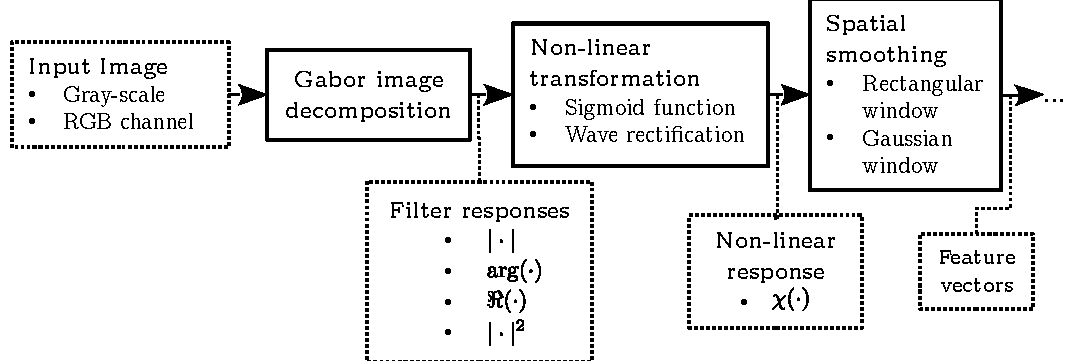
\includegraphics{general_pipeline_gabor_feature_extraction.pdf}
\caption{General pipeline for extraction of texture features using the Gabor filters}\label{fig:general_pipeline_gabor_feature_extraction}
\end{figure}

\subsection{Texture features for color images}

Most of the research work on texture has been done in the field of gray-scale images with homogeneous textures. In consequence, the first and simplest way to obtain texture features from color images is to transform it into a gray-scale image. This strategy favors the acceleration of feature calculation because we work with scalar values instead of vectors. However, despite the good results in images with homogeneous gray-scale textures, reducing channels for a natural color image with non-homogeneous textures does not ensure the generation of representative texture features for a colored real-world image containing non-homogeneous textures.

This idea is based on the relationship principle that have the texture and color in a real image and how we use this information. Certain works in the literature on the analysis of homogeneous color textures consider that the variation of the spatial structure (texture) and the distribution of the image are independent cues, however, we differ from this point of view and we consider that  color and texture information in a image are a joint phenomenon. For example, consider a texture image in the $RGB$ color space, where its gray-scale transformation represents the levels of red, green, and blue at a single luminance value $Y$ obtained with conversion equation of the ITU Rec. 709.

\begin{equation}\label{eq:color2gray_formula}
    Y = 0.2126 R + 0.7152 G + 0.00722 B
\end{equation}
 
Although there is some texture information in the color input image, in the case of isoluminant colors or colors with the same luminance value, the transformation $Y$ leads to a minimization or lost, in the worst case, of textures generated by the color changes. This is because the non-homogeneous textures in a color image are not only generated by lighting variations, but also by variations in chromaticity. Moreover, the real world scenes are in color and contain non-homogeneous textures.

\textit{Idea to develope:} Illustrate the effect of compute unichrome features in the gray-scale and the RGB space for a color image.

In both cases, the choice of color space for the representation of the texture is necessary. We can represent the image in a primary color space such as the $RGB$, in a Luminance-Chrominance based color space such as the $LAB$ or the $LUV$, or in a perceptual color space such as the $HSV$ or the $HLS$. 

A popular technique based on the $RGB$ primary color space consist in applying the Gabor decomposition in each image channel to obtain a vector of unichromatic features. The filter output represents the features of each color channel independently, so this strategy does not involve the correlation between $RGB$ band colors. This might be corrected using the opponent color model based on the human color vision theory. In this case each unichromatic feature vector ($RGB$-feature) is multiplied and normalized by the feature vector of its opponent color to include the correlation between color channels, which implies an extra post-processing step in the extraction pipeline of features.

One way to avoid the post-processing stage is to first transform the color image in a color space that handles the coupling between the color channels rather than separating them as components of the color space, and then performing the Gabor decomposition. One possible option for the color representation is the quaternion framework \cite{Sangwine.Ell:VISP:2000}. This encodes the color value of each pixel in a pure quaternion, where the real component is set to zero and the three imaginary components represent the color band such as $I(x, y) = R (x, y) i + G (x, y) j + B (x, y) k $. This 3-component vector representation yields a system which has well-defined mathematical operations, such as Quaternion Fourier Transform, which makes possible the Gabor image decomposition by means of the Quaternion Gabor Filters (QBF) \cite{Subakan.Vemuri:EMMCVPR:2009}. However, when using quaternion values, the non-existing commutativity has to be taken into account, in addition, the QGF does not support any physic interpretation of what is measured.





% We then propose to analyze the textures of an image from the spectral decomposition of the channels of a color image. Such an analysis could be performed with the image represented in some classic color space such as RGB or HSV. However, we have found that the analysis of the texture per channel in any of these color spaces does not really reflect the textures generated by the color changes. To illustrate this effect, imagine an image that contains a vertical texture generated from the variation between the pure colors red, green, and blue (RGB).

\section{Two-channel complex image representation}

From the previous section, it is clear that the luminance information is a cue in obtaining texture features, however, the chrominance also plays an important role. We can obtain this information using the two-complex channels form. This representation contains the pure luminance $L$ values in a real channel while the chrominance $C$ is contained in a complex channel. This complex channel can be obtained from the components of the $LAB$ or the components of $HSV$ / $HLS$ color spaces prior to a transformation of the image from the $RGB$ space.

Thus, the complex chrominance channel in its exponential form is defined as  

\begin{equation}\label{eq:chrominance_hsv}
    C(x,y) = S(x,y) e^{iH(x,y)}
\end{equation}
where $H$ is the hue and $S$ is the saturation value obtained after the $RGB$ to $HLS$ transformation. While the combined chrominance function for $LAB$ is defined as

\begin{equation}\label{eq:chrominance_lab}
    C(x,y) = A(x,y) + iB(x,y)
\end{equation}
where $A$ and $A$ are two chroma variables obtained from $RGB$ to $LAB$ transformation. 

We obtain a complex representation of chrominance content of the image whose spectrum is interesting to analyze in order to characterize the spatial variations of the chromatic part of the image. 

\section{Spectral decomposition of color images}

